\title{CS 613 - Machine Learning}
\author{
        Assignment 2 - Logistic Regression \\
        Robert Thompson \\
}
\date{}
\documentclass[12pt]{article}

\usepackage[margin=0.7in]{geometry}
\usepackage{float}
\usepackage{amsmath}
\usepackage{graphicx}
\graphicspath{ {./images/} }

\begin{document}
\maketitle

\section{Theory}
\begin{enumerate}
\item For the function $J=(x_1 w_1 -5x_2 w_2-2)^2$, where $w=[w_1, w_2]$ are our weights to learn:
    \begin{enumerate}
    \item What are the partial gradients, $\frac{\partial J}{\partial w_1}$ and $\frac{\partial J}{\partial w_2}$?
        \begin{enumerate}
            \item Partial Gradient of $\frac{\partial J}{\partial w_1}$:
            \begin{enumerate}
            \item Chain Rule\\
            $\frac{\partial J}{\partial w_1}$ $=2(x_1w_1 - 5x_2w_2-2)$ $\frac{\partial J}{\partial w_1}$ $(x_1_w_1 - 5x_2_w_2 -2)$ 
            \item Sum/Difference Rule\\
            $\frac{\partial J}{\partial w_1}$$(x_1_w_1 - 5x_2_w_2 -2)$ = $\frac{\partial J}{\partial w_1}$ $(x_1w_1)$ - $\frac{\partial J}{\partial w_1}$$(5x_2w_2)$ - $\frac{\partial J}{\partial w_1}$$(2)$ \\
            $\frac{\partial J}{\partial w_1}$$(x_1w_1)$ = $x_1$ \\
            $\frac{\partial J}{\partial w_1}$$(5x_2w_2)$ = $0$ \\
            $\frac{\partial J}{\partial w_1}$$(2)$ = $0$ \\
            $= x_1 - 0 - 0$ \\
            $= x_1$
            \item Partial Gradient
            $\frac{\partial J}{\partial w_1}$ = $2x_1(x_1w_1 - 5x_2w_2 -2)$
            \end{enumerate}
        \end{enumerate}
        
        \begin{enumerate}
            \item Partial Gradient of $\frac{\partial J}{\partial w_2}$:
            \begin{enumerate}
            \item Chain Rule\\
            $\frac{\partial J}{\partial w_2}$ $=2(x_1w_1 - 5x_2w_2-2)$ $\frac{\partial J}{\partial w_2}$ $(x_1_w_1 - 5x_2_w_2 -2)$ 
            \item Sum/Difference Rule\\
            $\frac{\partial J}{\partial w_2}$$(x_1_w_1 - 5x_2_w_2 -2)$ = $\frac{\partial J}{\partial w_2}$ $(x_1w_1)$ - $\frac{\partial J}{\partial w_2}$$(5x_2w_2)$ - $\frac{\partial J}{\partial w_2}$$(2)$ \\
            $\frac{\partial J}{\partial w_2}$$(x_1w_1)$ = $0$ \\
            $\frac{\partial J}{\partial w_2}$$(5x_2w_2)$ = $5x_2$ \\
            $\frac{\partial J}{\partial w_2}$$(2)$ = $0$ \\
            $= 0 - 5x_2 - 0$ \\
            $= -5x_2$
            \item Partial Gradient
            $\frac{\partial J}{\partial w_2}$ = $-10x_2(x_1w_1 - 5x_2w_2 -2)$
            \end{enumerate}
        \end{enumerate}
    \item What are the value of the partial gradients given current values of $w=[0, 0], x=[1, 1]$?
        \begin{enumerate}
            \item Let $\frac{\partial J}{\partial w_1}$ = $2x_1(x_1w_1 - 5x_2w_2 -2)$
            \begin{enumerate}
            \item Plugin $w=[0, 0], x=[1, 1]$\\
            $\frac{\partial J}{\partial w_1}$ = $2(1)(1 * 0 - 5(1)(0) -2)$
            \item Partial Gradient Value of $\frac{\partial J}{\partial w_1}$ = $-4$
            \end{enumerate}
            
            \item Let $\frac{\partial J}{\partial w_2}$ = $-10x_2(x_1w_1 - 5x_2w_2 -2)$
            \begin{enumerate}
            \item Plugin $w=[0, 0], x=[1, 1]$\\
            $\frac{\partial J}{\partial w_2}$ = $-10(1)(1 * 0 - 5(1)(0) -2)$
            \item Partial Gradient Value of $\frac{\partial J}{\partial w_2}$ = $20$
            \end{enumerate}
        \end{enumerate}
    \end{enumerate}
\end{enumerate}
\newpage

\section{Spambase Logistic Regression Classier}\label{naive}

\begin{enumerate}
   \item Plot of Training and Validation Log Loss as a Function of the Epoch
   \begin{itemize}
     \item Learning Rate: $0.1$
     \item Epochs: $10,000$
     \item Stability Constant: $10e-7$
   \end{itemize}
    \begin{figure}[H]
        \begin{center}
        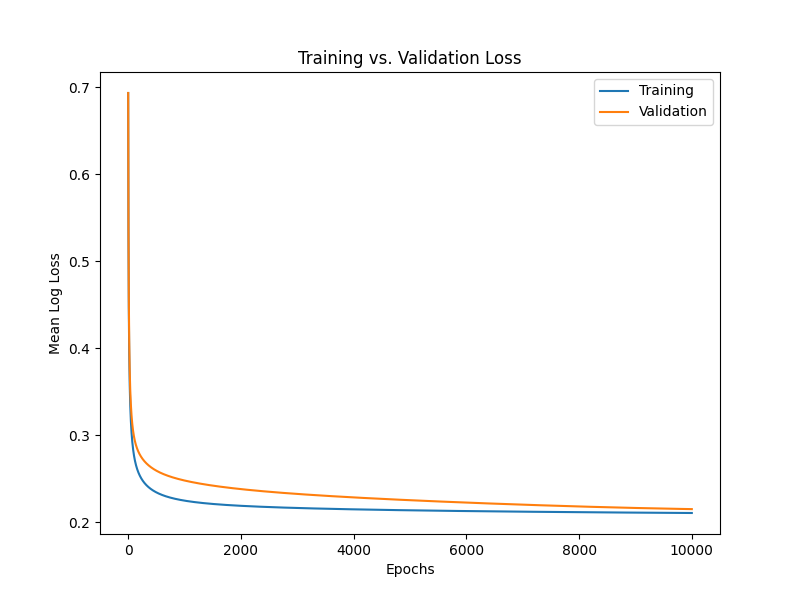
\includegraphics{images/training_validation_mean_log_loss.png}
        \label{GD}
        \end{center}
    \end{figure}
   \item Training Statistics
   \begin{itemize}
     \item Precision: $0.9267676767676768$
     \item Recall: $0.8900565885206144$
     \item F-Measure: $0.9080412371134021$
     \item Accuracy: $0.9272905119008803$
   \end{itemize}
   \item Validation Statistics
   \begin{itemize}
    \item Precision: $0.9092495636998255$
     \item Recall: $0.9045138888888888$
     \item F-Measure: $0.9068755439512619$
     \item Accuracy: $0.9302477183833116$
   \end{itemize}
   \item Training and Validation Precision-Recall Graph
   \begin{itemize}
     \item Learning Rate: $0.1$
     \item Epochs: $10,000$
     \item Stability Constant: $10e-7$
   \end{itemize}
    \begin{figure}[H]
        \begin{center}
        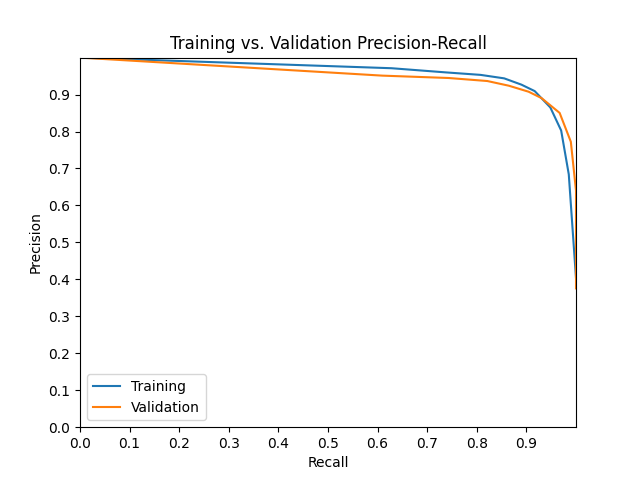
\includegraphics{images/training_validation_precision_recall_graph.png}
        \label{GD}
        \end{center}
    \end{figure}
\end{enumerate}

\newpage
\section{Logistic Regression for Multi-Class Classification}\label{naive}
\begin{enumerate}
   \item Validation Accuracy: $0.96$
   \item Validation Confusion Matrix
   \begin{itemize}
     \item $
        \begin{bmatrix}
        19 & 0 & 0\\
        0 & 15 & 2\\
        0 & 0 & 14
        \end{bmatrix}\\$
   \end{itemize}
\end{enumerate}
\end{document}